\begin{abstract}
This paper is written as a part of the course CS 140 "Parallel Scientific Computing" at UCSB and is on implementation of a parallel program that simulates motion in the n-body problem, where the n bodies resembles planets in a galaxy.
\end{abstract}

\section{Implementation}
The code was implemented for parallel processors using the MPI library for C. The main() function is called from nBody.c which initializes the MPI functions, collects planet data and calculates the nBody problem. The program can generate parameters, mass and initial positions and velocities for the n planets in two different ways. Either it generates randomly distributed values around realistic parameter values, or it reads from a file input.txt redirected to standard input. When reading from the file input.txt, the data is read by processor 0 and then distributed to all other processors, while when generating random values each processor generates their values. When each processor has generated its parameter values for $\frac{n}{nprocs}$ planets the nbody() function starts calculating the n body problem. \\
\textbf{Nbody()}. In the nbody() function each processor with an even rank has 2 buffers used for communication, in order to first receive and then send, while the odd ranked processors has only one buffer. For each iteration of the numerical integration of the n-body problem, each processor calculates the effects between it's $\frac{n}{nprocs}$, then it uses a "Mary Go Round" routine where each processor's data goes to the processor with $rank=rank+1$ (except for processor 0 and processor nprocs-1). Further each processor's planets are updated with a new position and a new velocity using the simple numerical integration:

\begin{align}
\label{eq:}
 v_n&=v_{n-1}+a_n*T \\
p_n&=p_{n-1}+v_n*T
 \end{align}
Where $v, a, p$ and $T$ is the position, acceleration, velocity and time step respectively. \\




\textbf{Testing and Debugging}
For testing and debugging, the result from the calculations where compared to a matlab code, reading the input.txt using the same values for $T,n$ and $I$(number of iterations). This made
the testing easy, and proved the code successful. 

 \clearpage
\section{Performance}
The performance tests where done by running the code on Triton. The timing was done using MPI\_Wtime() which measured the running time of  the $nbody()$ function.
From Fig. \ref{fig:n}, Fig. \ref{fig:p} and Fig. \ref{fig:ef} on can see that the parallelization of the simulation had a great benefit for large problem sizes. In Fig. \ref{fig:ef} on can see that even with 64 processors, the parallel efficiency is 0.94. The "Mary Go Round" communication strategy then proves to be efficient. In comparison with assignment \# 2 where each processor had to communicate to processor 0, thus increasing the communication load on processor 0 with the increase in processors. In this algorithm each processor communicates only with two processors, regardless of the number of processors, and the sharing of data can run in parallel. 




\begin{figure}[h!] 
 \center 
 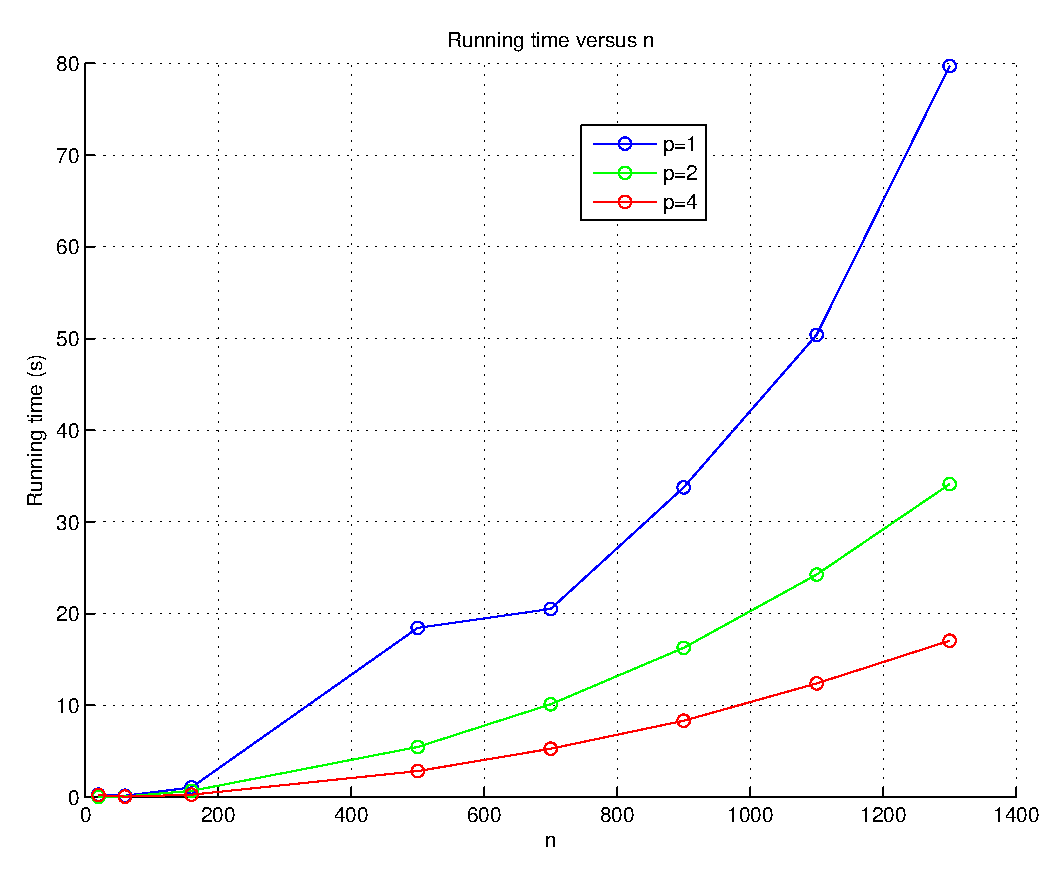
\includegraphics[scale=\figurescale]{\figurepath/running_times_n.eps}
 \caption{Plot of running times vs. problem size n (number of planets) for a different number of processors. The simulation where done over 500 iterations with a time step of 2000 \label{fig:n}}
 \end{figure}

\begin{figure}[h!] 
 \center 
 \includegraphics[scale=\figurescale]{\figurepath/running_times_p.eps}
 \caption{ Plot of running times vs. number of processors from 15 to 64, for 100 iterations of the n-body problem \label{fig:p}}
 \end{figure}

\begin{figure}[h!] 
 \center 
 \includegraphics[scale=\figurescale]{\figurepath/parallel_ef.eps}
 \caption{ Plot of the parallel efficiency vs. number of processors from 1 to 64. \label{fig:ef}}
 \end{figure}


\clearpage


\begin{table}
\caption{Table of running times in seconds for different problem size n and number of processors p}
\begin{tabular}{|l|l|l|l|l|l|l|l|l|}
\hline
 & n=20 & n=60 & n=160 & n=500 & n=700 & n=900 & n=1100 & n=1300 \\ \hline
p = 1 & 0.27376 & 0.16216 & 1.0743 & 18.465 & 20.523 & 33.781 & 50.418 & 79.698 \\ 
p = 2 & 0.039658 & 0.091980 & 0.68724 & 5.4764 & 10.0128 & 16.286 & 24.270 & 34.1266 \\ 
p = 4 & 0.23168 & 0.064689 & 0.28196 & 2.8403 & 5.2929 & 8.3341 & 12.400 & 17.061 \\
\hline
\end{tabular}
\end{table}



\begin{table}
\caption{Running times for a different number of processors, for problem size n=10000, with 100 iterations.}
\begin{tabular}{|l|l|l|l|l|l|l|l|}
\hline
nprocs & p = 1 & p = 16 & p = 20 & p = 25 & p = 40 & p = 50 & p = 64 \\  \hline
running time [s] & 800 & 51.036 & 40.788 & 32.927 & 20.517 & 16.692 & 13.302 \\
\hline
\end{tabular}
\end{table}








